\documentclass[ignorenonframetext,]{beamer}
\usepackage{amssymb,amsmath}
\usepackage{ifxetex,ifluatex}
\usepackage{fixltx2e} % provides \textsubscript
\ifxetex
  \usepackage{fontspec,xltxtra,xunicode}
  \defaultfontfeatures{Mapping=tex-text,Scale=MatchLowercase}
\else
  \ifluatex
    \usepackage{fontspec}
    \defaultfontfeatures{Mapping=tex-text,Scale=MatchLowercase}
  \else
    \usepackage[utf8]{inputenc}
  \fi
\fi
\usepackage{listings}
\usepackage{microtype}
\usepackage{syntax}
\usepackage{qtree}
% Comment these out if you don't want a slide with just the
% part/section/subsection/subsubsection title:
\AtBeginPart{\frame{\partpage}}
\AtBeginSection{\frame{\sectionpage}}
\AtBeginSubsection{\frame{\subsectionpage}}
\AtBeginSubsubsection{\frame{\subsubsectionpage}}
\setlength{\parindent}{0pt}
\setlength{\parskip}{6pt plus 2pt minus 1pt}
\setlength{\emergencystretch}{3em}  % prevent overfull lines
\setcounter{secnumdepth}{0}

\title{Identifying change patterns in software history}
\author{Jason Dagit \and Matthew Sottile}
\date{Galois, Inc}


\definecolor{javared}{rgb}{0.6,0,0} % for strings
\definecolor{javagreen}{rgb}{0.25,0.5,0.35} % comments
\definecolor{javapurple}{rgb}{0.5,0,0.35} % keywords
\definecolor{javadocblue}{rgb}{0.25,0.35,0.75} % javadoc
 
\newcommand\Small{\fontsize{8}{8.0}\selectfont}
\newcommand*\LSTfont{\Small\ttfamily\SetTracking{encoding=*}{-60}\lsstyle}
\lstset{language=Java,
%basicstyle=\ttfamily,
%% JED: Kill these lines if you want black&white
keywordstyle=\color{javapurple}\bfseries,
stringstyle=\color{javared},
commentstyle=\color{javagreen},
morecomment=[s][\color{javadocblue}]{/**}{*/},
morecomment=[l][\bfseries\color{javared}]{>-\ },
morecomment=[l][\color{javared}]{-\ },
morecomment=[l][\color{javagreen}]{+\ },
tabsize=4,
showspaces=false,
showstringspaces=false,
basicstyle=\LSTfont,
%frame=single, 
captionpos=b,
escapeinside={$}{$}}

%%\lstnewenvironment{java}[1][]{}{}
%%\lstnewenvironment{java}[1][]
%%{\lstset{#1,
%%         frame=single, 
%%         captionpos=b,
%%         basicstyle=\LSTfont,
%%         escapeinside={$}{$}}}
%%%%          basicstyle=\scriptsize\ttfamily}}
%%%%          basicstyle=\footnotesize\ttfamily}}
%%{}

\newcommand{\metavar}{$\square$}

\begin{document}
\frame{\titlepage}

\begin{frame}\frametitle{Motivation}

\textbf{Dream Tool:} Finds meaningful patterns in source code and edit
history to support people with the following roles:

\begin{itemize}
\item
  Language Designers
\item
  Programmers
\item
  Managers
\end{itemize}

\end{frame}

\begin{frame}[fragile]\frametitle{Motivation}

\begin{block}{Traditional line-based diff}

Pro: diff is very general and programming language agnostic

Con: diff is not structurally aware:

\begin{lstlisting}
if( foo ){           if( foo )
  bar;               {
}                      bar;
                     }
\end{lstlisting}

\end{block}

\end{frame}

\begin{frame}\frametitle{Motivation}

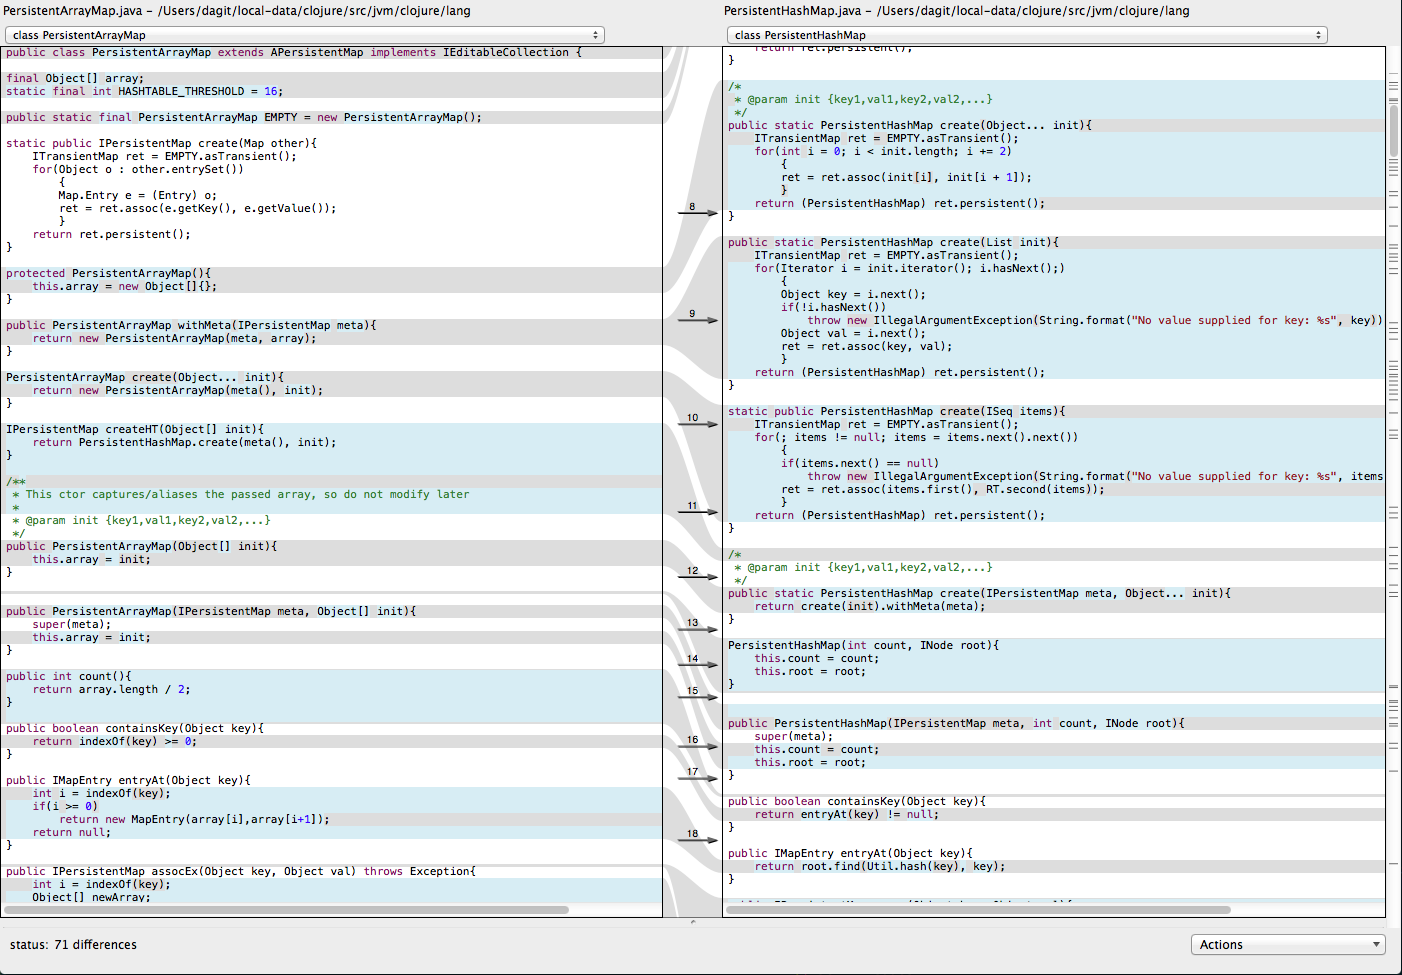
\includegraphics[height=0.8\textheight]{slide-figures/opendiff.png}

\end{frame}

\begin{frame}[fragile]\frametitle{Motivation}

What can language designers learn from patterns?

Common looping pattern with loop counter initialized to zero:

\begin{lstlisting}
for ($\metavar$ = 0; $\metavar$ < $\metavar$; $\metavar$) {
    $\metavar$
}
\end{lstlisting}

\begin{itemize}
\item
  Highlights language features that get used together
\item
  We also want to see how source code \emph{changes}
\end{itemize}

\end{frame}

\begin{frame}[fragile]\frametitle{Motivation}

How can programmers benefit from patterns?

Before:

\begin{lstlisting}
if( lock.acquire($\metavar$) ){
  $\metavar$
}
\end{lstlisting}

After:

\begin{lstlisting}
while( lock.acquire($\metavar$) ){
  $\metavar$
}
\end{lstlisting}

\begin{itemize}
\item
  Similar edits to two or more files $\Rightarrow$ might be a related
  change
\item
  Directs our attention to take a closer look
\item
  \emph{Only} a heuristic arugment, but humans are good at working with
  such information
\end{itemize}

\end{frame}

\begin{frame}\frametitle{Approach}

\textbf{Key Idea:} We can find \emph{structural patterns} by
generalizing \emph{sufficiently similar} difference trees.

\begin{itemize}
\item
  Difference trees computed using structural diff of AST
\item
  Similarity is measured using a tree edit distance score
\item
  Generalization is accomplished through antiunification
\end{itemize}

\end{frame}

\begin{frame}\frametitle{Workflow}

\begin{center}

  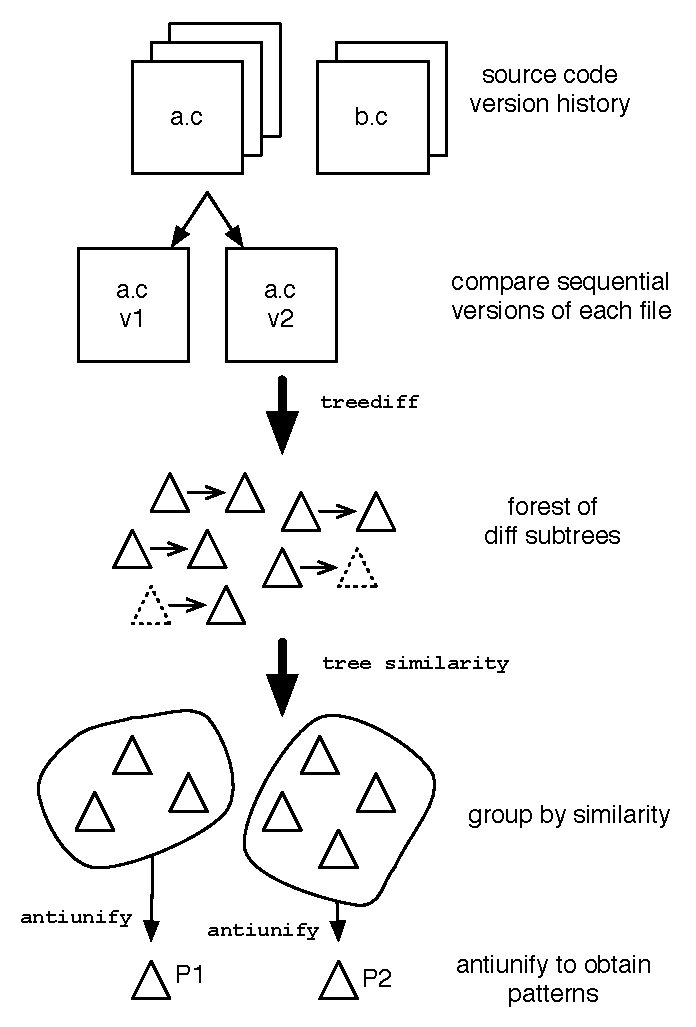
\includegraphics[height=0.8\textheight]{figures/workflow.pdf}

\end{center}

\end{frame}

\begin{frame}\frametitle{ATerms}

\setlength{\grammarindent}{8em}

\begin{grammar}
<aterm> ::= `AAppl' $\langle$string$\rangle$ $\langle$aterm-list$\rangle$
\alt `AList' $\langle$aterm-list$\rangle$
\alt `AInt' $\langle$int$\rangle$

<aterm-list> ::= $\langle$aterm$\rangle$ $\langle$aterm-list$\rangle$
\alt $\epsilon$
\end{grammar}

\begin{itemize}
\item
  Generic tree structure
\item
  Easy to modify parsers to generate ATerms
\end{itemize}

\end{frame}

\begin{frame}\frametitle{Structural Diff Example}

\[
treediff\left(\raisebox{1.5em}{\Tree[.A [.B ] [.C ]]},\raisebox{1.5em}{\Tree[.A [.B [.D ] ] [.F ]]}\right) = \raisebox{1.5em}{\Tree[.A [.B [.lefthole(D) ] ] [.mismatch(C,F) ]]}
\]

\end{frame}

\begin{frame}\frametitle{Similarity Grouping}

We define the similarity score by:

\[\Delta(t_a, t_b) := \frac{min(treediff(t_a, t_b),treediff(t_b, t_a))}{max(|t_a|,|t_b|)}\]

Distance matrix $D$ given by $D_{ij} = \Delta(t_i, t_j)$.

\end{frame}

\begin{frame}\frametitle{Similarity Grouping}

\begin{center}
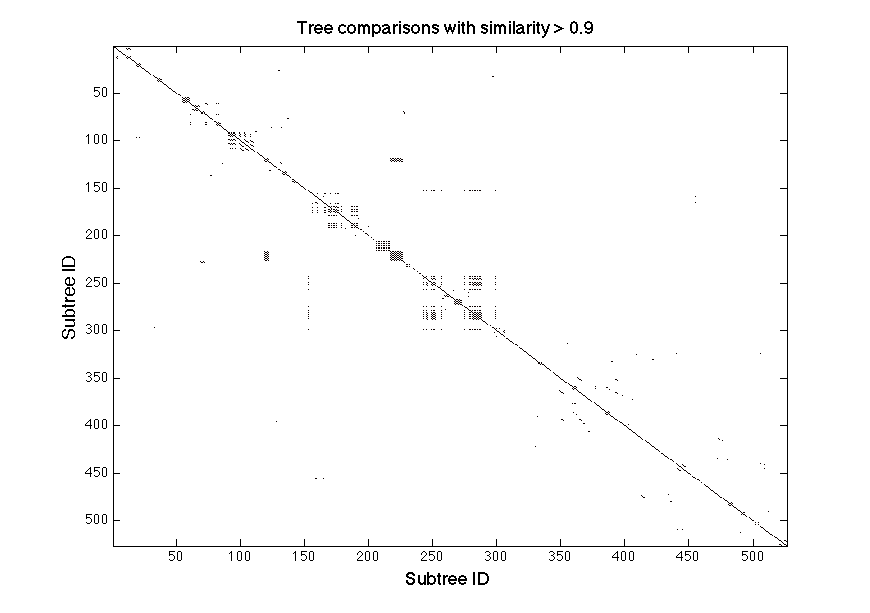
\includegraphics[width=0.9\textwidth]{figures/distmatrix-0-9.png}

Similarity groups from the ANTLR repository with similarity threshold greater than 0.9
\end{center}

\end{frame}

\begin{frame}\frametitle{Clojure}

\begin{center}
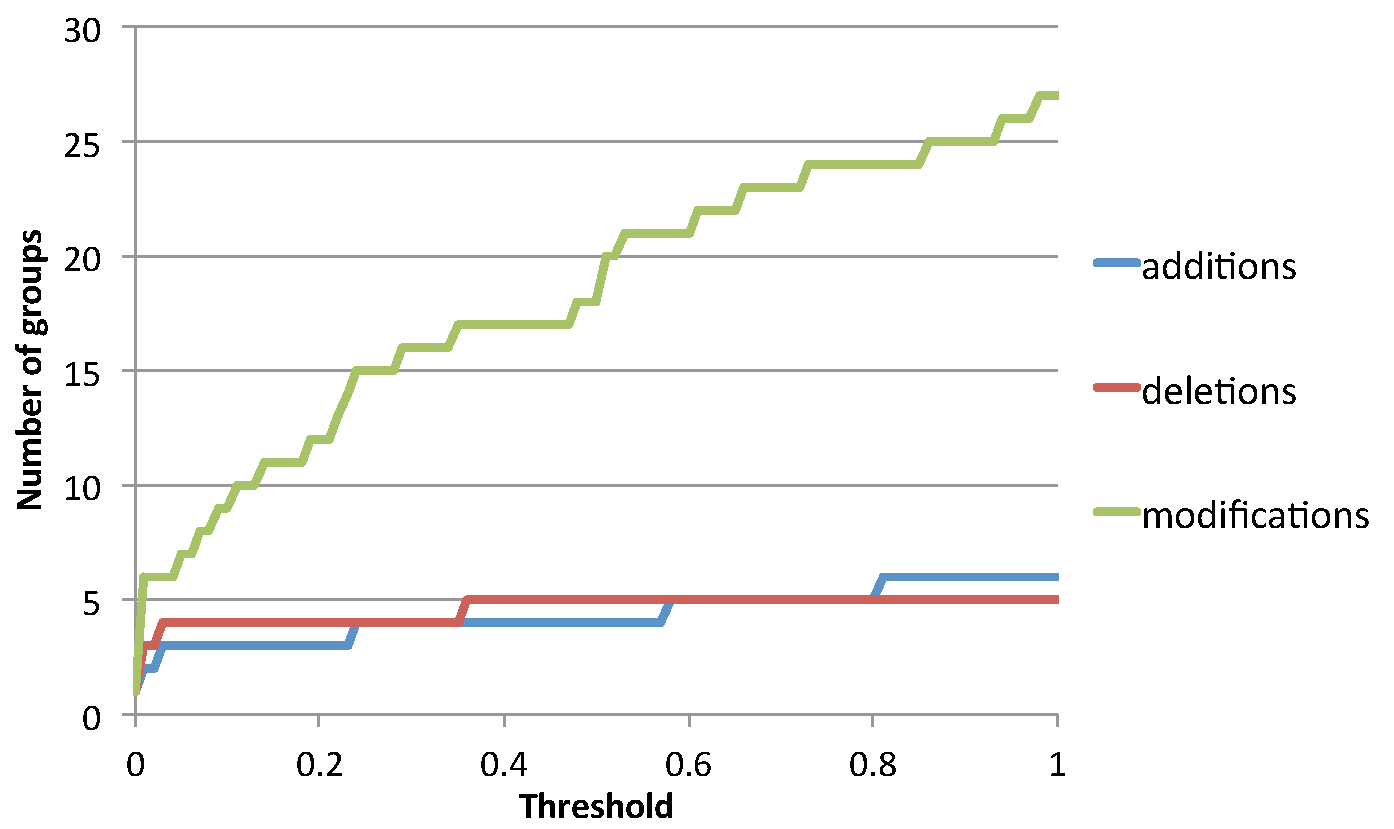
\includegraphics[width=\textwidth]{figures/clojure-number-of-modifications.pdf}


Number of additions, deletions, and modifications by threshold for the Clojure source.
\end{center}

\end{frame}

\begin{frame}\frametitle{ANTLR}

\begin{center}
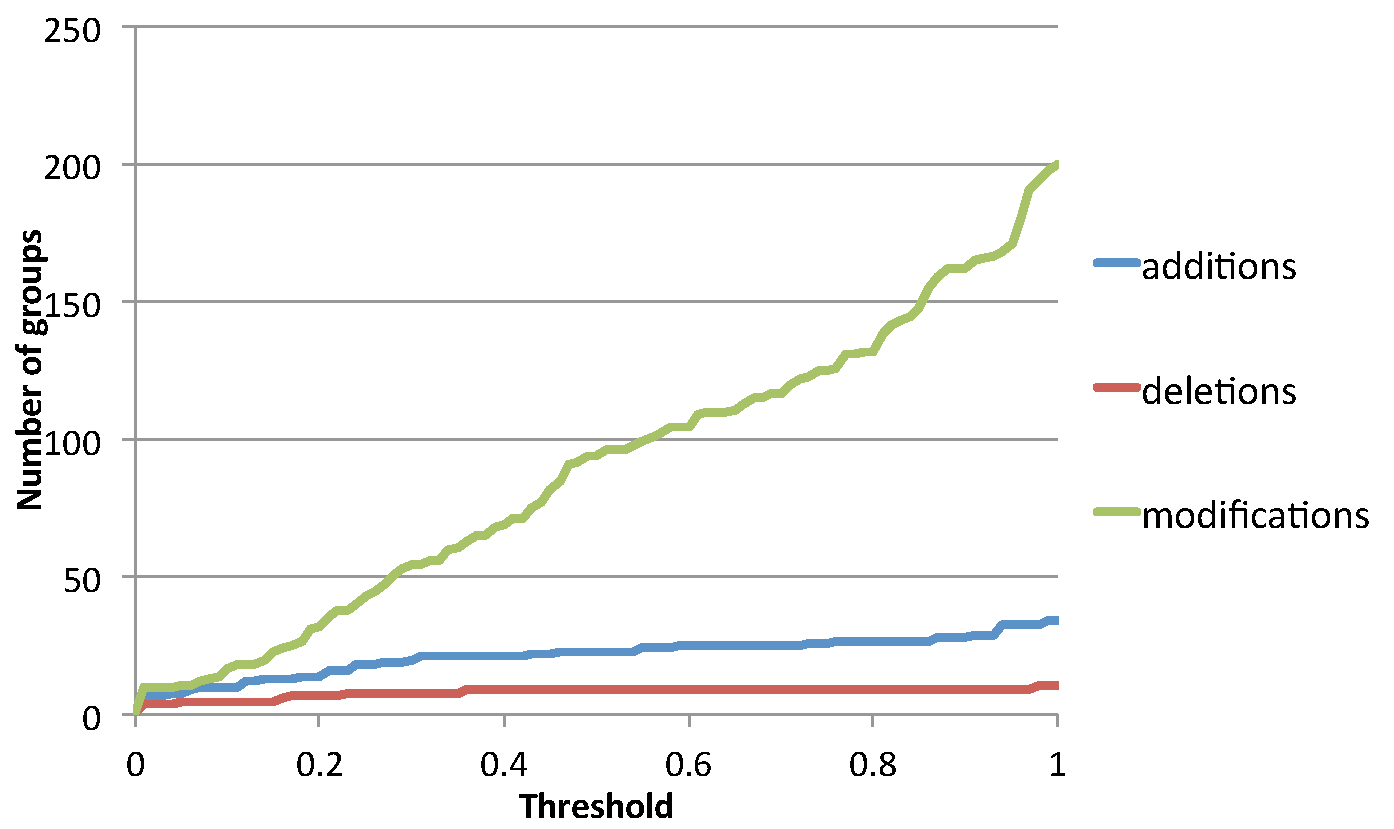
\includegraphics[width=\textwidth]{figures/antlr-number-of-modifications.pdf}

Number of additions, deletions, and modifications by threshold for the ANTLR source.
\end{center}

\end{frame}

\begin{frame}\frametitle{Antiunification Example}

\[
au\left(\raisebox{1.5em}{\Tree[.A [.B ] [.C ]]},\raisebox{1.5em}{\Tree[.A [.B [.D ]] [.F ]]}\right)
  = \left(\raisebox{1em}{\Tree[.A [.?_1 ] [.?_2 ]]},subst_l ,subst_r \right)
\]

where,

\begin{align*}
subst_l &= \{?_1 := B, ?_2 := C\} \\
subst_r &= \{?_1 := \raisebox{0.5em}{\Tree[.B [.F ]]}, ?_2 := F\}
\end{align*}

\end{frame}

\begin{frame}[fragile]\frametitle{Patterns as a function of threshold}

Generic Loop pattern:

\begin{lstlisting}
for ($\metavar$ = $\metavar$; $\metavar$ < $\metavar$; $\metavar$) {
    $\metavar$
}
\end{lstlisting}

Increase similarity requirement and the loop counter is initialized to
zero:

\begin{lstlisting}
for ($\metavar$ = 0; $\metavar$ < $\metavar$; $\metavar$) {
    $\metavar$
}
\end{lstlisting}

Increase it again and the loop termination criteria becomes more
specific:

\begin{lstlisting}
for ($\metavar$ = 0; $\metavar$ < $\metavar$.$\metavar$; $\metavar$) {
    $\metavar$
}
\end{lstlisting}

\end{frame}

\begin{frame}[fragile]\frametitle{Example from Clojure: Related edits}

\begin{lstlisting}
 public Object kvreduce(IFn f, Object init){
     for(int i=0;i < array.length;i+=2){
         init = f.invoke(init, array[i], array[i+1]);
-           if(RT.isReduced(init))
-                   return ((IDeref)init).deref();
         }
     return init;
 }
\end{lstlisting}

\begin{lstlisting}
 public Object kvreduce(IFn f, Object init){
-    for(INode node : array){
-        if(node != null){
+    for(INode node : array)
+        {
+        if(node != null)
             init = node.kvreduce(f,init);
-                if(RT.isReduced(init))
-                        return ((IDeref)init).deref();
-               }
-           }
+        }
     return init;
 }
\end{lstlisting}

\end{frame}

\begin{frame}\frametitle{Shortcomings:}

\begin{itemize}
\item
  Bias in dynamic programming of Yang's algorithm
\item
  We only consider structural patterns
\item
  Not semantically aware
\end{itemize}

\end{frame}

\begin{frame}\frametitle{}

\Large

\begin{center}
 Thank you!
\end{center}

\end{frame}

\end{document}
